\textbf{RT-PCR tests:} \hfill real time polymerase chain reaction
\begin{itemize}
    \item Amplification of nucleic acids is done through cycles of \textbf{DNA elongation} using \textbf{DNA polymerase} (temperature controlled)
    \item Steps: DNA denaturation, primer annealing, elongation of new DNA strand
    \item At each cycle, the number of DNA fragments doubles (measured \textbf{optically with fluorescent dye})
    \item Higher \textbf{sensitivity} than lateral flow tests
\end{itemize}

\textbf{Lateral flow tests:} \hfill rapid antigen tests
\begin{itemize}
    \item \textbf{Detection of proteins} (antigens) through
immobilization of a \textbf{receptor-nanoparticle
complex} on a substrate.
    \item \textbf{Antibodies bind to antigens} in the sample and
\textbf{antigens} simultaneously \textbf{bind} to capture \textbf{antibodies} immobilized on \textbf{test line}.
    \item The \textbf{antigen} is sandwiched between the \textbf{capture antibody} and the \textbf{detection complex}.
    \item Signal depends on: the amount of virus, flow,
diffusion of antigen proteins and kinetics of
reception-antigen binding.
\end{itemize}
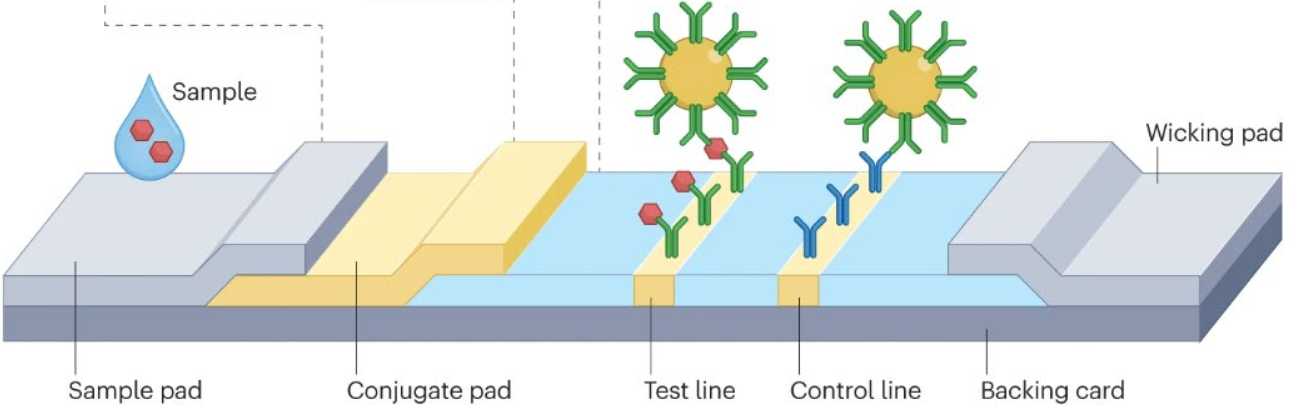
\includegraphics[width=38mm]{src/Images/antigen_test.png}
